\chapter{Risk factors for not completing a degree} \label{chap:3}

The path from enrolment to graduation is never entirely predictable. Some promising students end up failing or deciding to do something else. Some students succeed despite disadvantage and the obstacles in their way.

Despite this uncertainty, going to university is not a lottery in which anything might happen. Statistical analysis of university students shows that some factors and characteristics are signs of high risk of never getting a degree, and other factors and characteristics are signs of low risk.

Past academic achievement is a useful guide to future academic achievement. Students with a high ATAR have good prospects of completing university, while students with ATARs below 60 have a 40 per cent risk of not completing university within eight years, after taking account of a wide range of other characteristics. Similarly, students who have failed subjects in the past are less likely to complete than students who never fail any subjects.

While academic ability is essential, so too is the time needed to complete course requirements. Part-time study is the single biggest risk for non-completion, largely because most part-time students have other major responsibilities at home and at work.

\section{Learning from the experience of others}\label{sec:3.1}

The mutual selection process involves some uncertainty that can only be resolved by enrolling and seeing how it turns out. But students and universities can also learn from the experiences of others. Statistical analysis of student outcomes can identify personal or study factors that affect completion prospects. These can inform student and university decision-making.

This report draws on an analysis of students who started a bachelor degree at a public university between 2006 and 2008, and tracks them over eight years. It uses enrolment data collected by the Department of Education and Training. \Vref{fig:table1} summarises the variables included in the analysis. The starting hypothesis was not that these attributes necessarily cause a student to complete or not complete a degree, but that they might be associated with factors that more directly affect outcomes. These factors include academic ability, motivation, persistence, time put into study, study practices, financial support, social support, academic support and teaching quality.

                % "Table 1"
                \begin{figure}
                    \caption{The student and course characteristics used to analyse completion prospects \label{fig:table1}}%
                    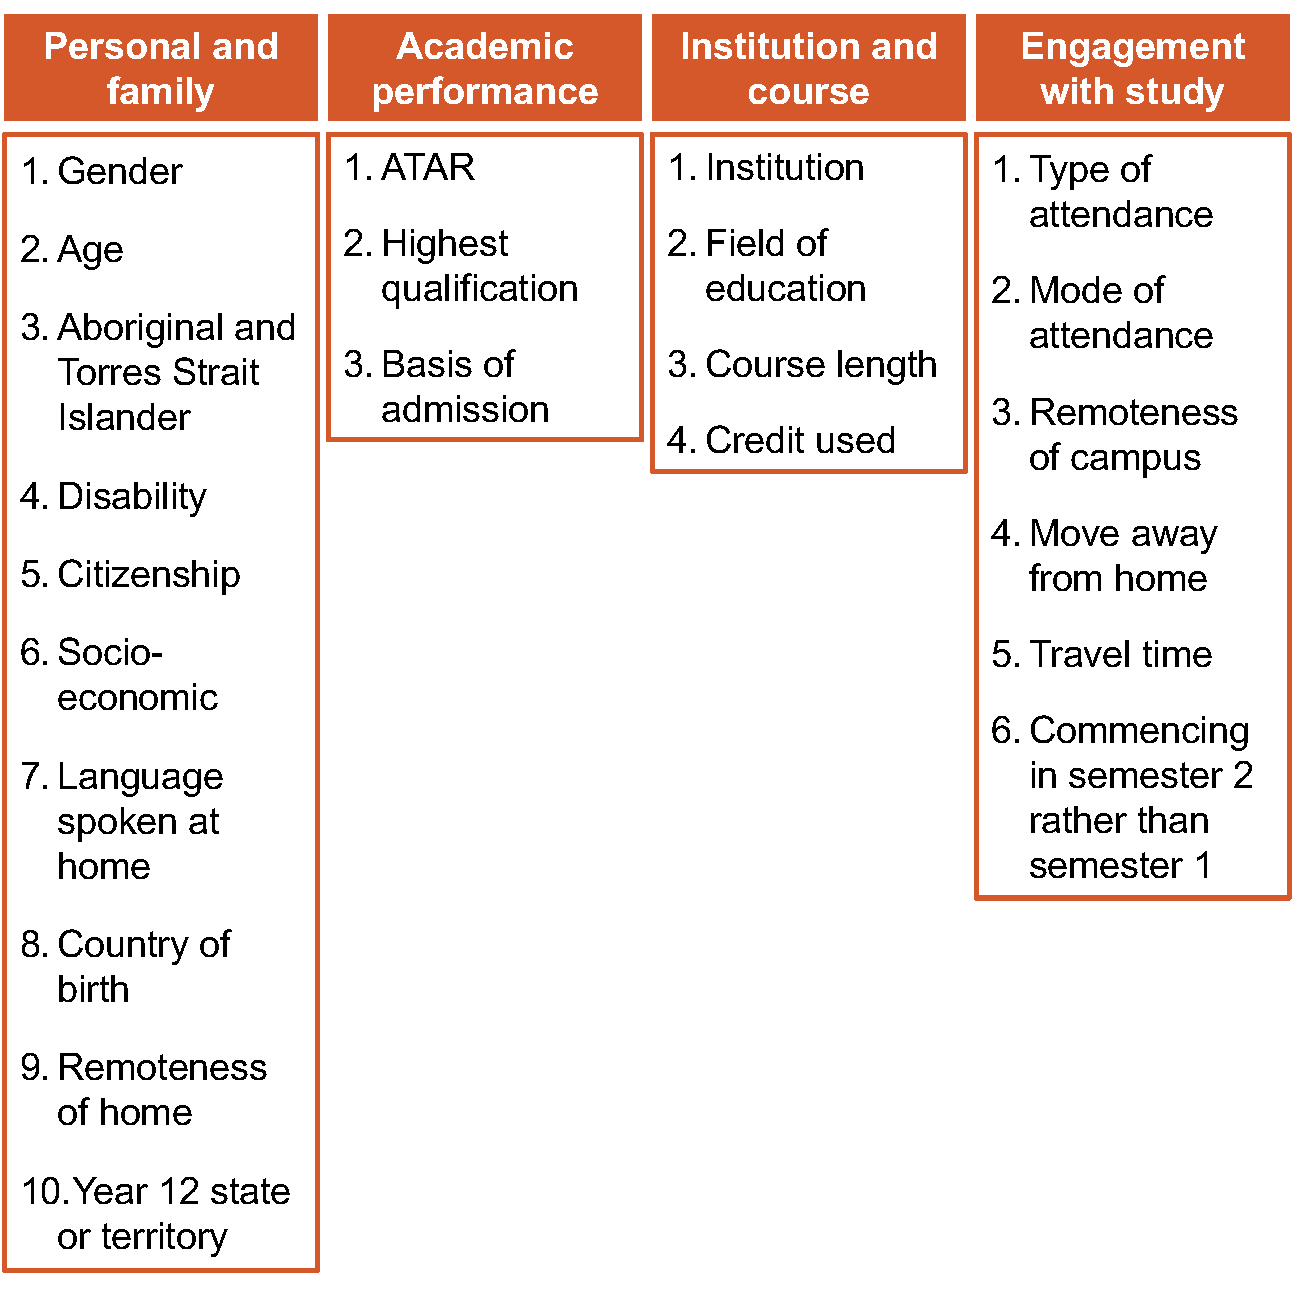
\includegraphics[page=1]{atlas/selection_deck_halfpage.pdf} 
                    \notes{A subject is assumed to equal 0.125 EFTSL\@. For further detail of each variable, see the background paper, \textcite{Cherastidtham2018a}}
                \end{figure}


This risk analysis aims to identify how each factor in isolation affects the risk of not completing. For example, many part-time students are also mature age, and many lower-ATAR students also have a lower socio-economic status. For student and university decision-making, it is important to work out the relative importance of each factor. In some cases, attributes that look high-risk in isolation are low-risk when other factors are taken into account.

The most significant predictive factors are prior academic performance and part-time study, because of their substantial influence on completion prospects, and because they affect many students. Subsequent sections of this chapter examine them in more detail. Most other variables listed in \Cref{fig:table1} have, in isolation, a modest, small, or no effect on completion rates, or affect only small numbers of students. But when combined with other risk factors they can be important to student and university decision-making. They are outlined only briefly in this chapter. A background paper, \emph{University attrition: what helps and what hinders university completion?}, discusses them in more detail.\footcite[][]{Cherastidtham2018a}


\subsection{Academic performance }\label{subsec:3.1.1}

Every university includes academic performance as part of its admission criteria. Most media attention focuses on ATAR, which ranks school leavers by their academic results. In recent years, about 40 per cent of commencing bachelor-degree students have been admitted based on their secondary education, although not always using their ATAR\@. Nearly as many students again are admitted based on prior vocational or higher education, so their academic preparation also needs to be closely examined.

ATAR incorporates the effects of ability and effort in school. These attributes are important at university as well, so it is unsurprising that ATAR levels are linked to completion rates.\footnote{\textcite{Cardak2017} also found a strong positive impact of ATAR using the 2006 Longitudinal Survey of Australian Youth (LSAY) data. With LSAY data, \textcite{Lim2011} found a positive effect of Programme for International Student Assessment (PISA) scores on completion. PISA is an international test of the skills and knowledge of 15-year-olds.} \Vref{fig:13} shows the risk of not completing by ATAR band, after controlling for other factors in the analysis.

Commencing students with ATARs of 90 or above have a low risk -- below 20 per cent. This means 2-in-10 students with an ATAR of 90 or above, who otherwise have an average background representative of all commencing students, will not complete with eight years. The risk is marginally higher for men than women, but both are low risk. The risk of not completing rises as ATAR falls among students with otherwise similar backgrounds. For students with an ATAR of between 70 and 79, the risk is above 30 per cent. And for students with an ATAR of below 60, the risk rises to twice the level for students with an ATAR of 90 or above, to about 40 per cent.

                \doublecolumnfigure {
               % Figure 13
                %\begin{figure}
                    \caption{High-ATAR students are much more likely to complete a degree\label{fig:13}}%
                    \units {Risk of not completing within eight years, controlling for other factors, per cent}
                    \includegraphics[page=18]{atlas/selection_chartdeck.pdf} 
                    \noteswithsource{Predictive margins are shown. This means, for example, that controlling for all the other characteristics in the analysis, a student with an ATAR between 70 and 79 has a non-completion risk 15 percentage points higher than a student with an ATAR of 90 or above. See the background paper, \textcite{Cherastidtham2018a} for further detail.}
                    {Grattan analysis of \textcite{DepartmentofEducationandTraininga}}
                %\end{figure}

                }{

                % Figure 14
                %\begin{figure}
                    \caption{People who have previously succeeded in higher education are more likely to complete \label{fig:14}}%
                    \units {Risk of not completing within eight years, controlling for other factors, per cent}
                    \includegraphics[page=19]{atlas/selection_chartdeck.pdf} 
                    \noteswithsource{Based on a sub-sample of students commencing in 2008. Only includes students admitted based on incomplete higher education and who were enrolled in 2007. Predictive margins are shown. See also the background paper, \textcite{Cherastidtham2018a}}
                    {Grattan analysis of \textcite{DepartmentofEducationandTraininga}}
                %\end{figure}
                }

Nearly 20 per cent of commencing bachelor degree students have incomplete higher education. Changing courses is a significant aspect of the mutual selection process into university.\footnote{In recent years, 17.5 per cent of commencing bachelor degree students have an incomplete higher education course as their highest previous education. This is not necessarily their basis of admission: \textcite{DepartmentofEducationandTraininga}.} 
At least for students who complete a full year of study before switching, changing courses does not of itself have a major negative effect on completion prospects. But previous university performance does predict their risk of not completing. Students who passed all their subjects in the year prior to changing courses have a relatively low non-completion risk of about 20 per cent. Those who have previously failed subjects are less likely to complete their new course. Students who have failed half their subjects have a non-completion risk of more than 40 per cent (\Cref{fig:14}).\footnote{In recent years, 1.5-to-1.8 per cent of commencing bachelor degree students failed half or more of the subjects they took in the previous year: ibid.}

People who have previously completed vocational or sub-bachelor qualifications are more likely to complete a higher education degree than otherwise. About 10 per cent of students admitted have a completed vocational qualification and another 4 per cent have a completed higher education diploma or associate degree.\footnote{Ibid.} 
Students admitted with a vocational qualification have a non-completion risk of 28 per cent, and students with a higher education diploma or associate degree have a risk of 27 per cent.\footnote{Diplomas include pathway courses that usually have a remedial element, as well as specialised courses such as diplomas of languages. However, language diplomas are typically taken concurrently with a bachelor degree, and so are unlikely to be reported as a highest prior qualification.} 
These are slightly lower risks than for all students whose highest educational attainment is Year 12. Higher education diploma and associate degree students usually had relatively low ATARs.\footnote{For example, in 2015 median ATARs for commencing students were: 80 for bachelor pass degree students who finished school in 2014, 65 for associate degree students, and 52 for diploma or advanced diploma students: \textcite{DepartmentofEducationandTraining2017n}.} They are more likely to complete higher education degrees than would be expected given their ATAR\@. It is probable that they improve academically during their diploma or associate degree; and these courses also screen out students who are unlikely to succeed in higher education.

\subsection{Part-time study}\label{subsec:3.1.2}

About 18 per cent of commencing domestic bachelor degree students begin their studies part-time.\footnote{The official definition of part-time study is taking less than 75 per cent of the normal annual subject load of a full-time student.} 
For them, four subjects over a year is the most common study load, half the standard full-time level. About 20 per cent of commencing part-time students switch to full-time in second year, about 40 per cent remain part-time, and the rest do not continue with their studies.\footnote{Based on students commencing between 2006 and 2008.}

As this high departure rate shows, part-time students often do not persist. No other factor in the statistical analysis is more negative for completion prospects than part-time study. \Cref{fig:15} shows the risk of not completing is higher if students enrol in fewer subjects in their first year. Students who enrol in two subjects or fewer in their first year are least likely to complete, with more than a 60 per cent risk of not completing within eight years. The part-time students who do complete typically increase the number of subjects they take after first year.

The results for students with very few subjects require some caveats. As discussed in \Cref{sec:1.1} some newly-enrolled students are trying out university, without a firm intention to complete on the day they enrol. Taking one or two subjects can be an experiment with study: students who like it and pass continue; the others leave.\footnote{In a separate analysis, nearly 2 per cent of commencing bachelor pass degree enrolments enrolled in one subject between 2006 and 2015. Of those, 60 per cent were categorised as potentially trialling university -- with prior education of less than a bachelor degree and either increasing their study load or leaving university after first semester. Another possible category of students, although not one easily identifiable in the data, is students who always intended to be full-time but dropped most of their subjects prior to the census date, perhaps after realising that they had chosen the wrong course.} Departing students found out that university was not for them, at low cost.

Other students taking very few subjects may be seeking specific skills or knowledge without planning on taking a full degree. Universities offer not-for-award subjects for such students, but these attract no government subsidies and students must pay upfront fees. It is cheaper for the student to enrol in a course, and then drop out. Students who already have a degree and enrol in only one subject in a subsequent bachelor degree could be in this category.\footnote{In the separate analysis of one-subject bachelor pass degree enrolments (footnote 64), 6 per cent were classed as potentially in this group because they already had a bachelor degree or above and did not re-enrol in semester two after taking one subject: \textcite{DepartmentofEducationandTraininga}.}

Students taking three, four or five subjects a year are more likely to be aiming for a degree. \Vref{fig:15} shows that their risk of not completing within eight years is much lower than students taking one or two subjects a year. Students who take more than six subjects -- 75 per cent of a full year load -- in their first year are least likely to drop out, with a 22 per cent risk of not completing in eight years. They are likely to stay full-time; of the full-time commencing students in our analysis, less than 8 per cent enrolled part-time in any subsequent year. Full-time study maximises a student's chance of completing their course.

Even for students who start part-time, converting to full-time study is a valuable strategy for completion. Of the students who never enrol full-time, only 19 per cent complete a bachelor degree within eight years, with another 9 per cent still enrolled.\footnote{This figure does not control for other risk factors, meaning that factors and characteristics other than part-time study may contribute to this outcome.} At best, less than 30 per cent of continuously part-time students will complete a course.


                % Figure 15
                \begin{figure}
                    \caption{Studying part-time increases the risk of not completing, and the fewer subjects the higher the risk\label{fig:15}}%
                    \units {Risk of not completing within eight years, controlling for other factors, per cent}
                    \includegraphics[page=20]{atlas/selection_chartdeck.pdf} 
                    \noteswithsource{Predictive margins are shown. Based on subjects taken in the first two semesters. Six or more subjects in a year is regarded as full-time. See also the background report, \textcite{Cherastidtham2018a}.}
                    {Grattan analysis of \textcite{DepartmentofEducationandTraininga}}
                \end{figure}

                \doublecolumnfigure{
                % Figure 16
                %\begin{figure}
                    \caption{Part-time students are more likely than full-time students to work full-time\label{fig:16}}%
                    \units {Per cent of students by type of attendance, 2016}
                    \includegraphics[page=21]{atlas/selection_chartdeck.pdf} 
                    \noteswithsource{Including bachelor degree students at universities and other providers and all ages.}
                    {\textcite{ABS2016b}}
                %\end{figure}
                }{
                % Figure 17
                %\begin{figure}
                    \caption{Part-time students are much more likely to cite work and family responsibilities as reasons for considering leaving\label{fig:17}}%
                    \includegraphics[page=22]{atlas/selection_chartdeck.pdf} 
                    \noteswithsource{Health and stress is also a top reason, at about 30 per cent. Domestic bachelor-degree students. Data from 2012-2015.}
                    {\textcite{SocialResearchCentre/DepartmentofEducationandTraining}}
                %\end{figure}
                }


Many students study part-time because they are time poor. According to Australian Bureau of Statistics data, part-time students are more likely to work and to work longer hours than full-time students (\Vref{fig:16}). Median weekly working time is less than 10 hours for full-time students; for part-time students it is 30-to-39 hours. With work commitments, part-time students have less time available for study and engagement with other aspects of university life.\footnote{The lack of engagement is with other students rather than with academic staff, see \Cref{fig:17} and \textcite[][section~2.1]{Cherastidtham2018a}.} The Government's Student Experience Survey shows that part-time students disproportionately nominate paid-work as a reason they consider discontinuing (\Vref{fig:17}).

Adding to their time commitments, part-time students are also much more likely than full-time students to have young children. Among students aged 25-44, nearly 40 per cent of part-time students have a youngest child aged under 15, compared to about 25 per cent of full-time students.\footnote{Including bachelor degree students at universities and other providers; \textcite{ABS2016b}.} Among students considering leaving university, part-time students are twice as likely as full-time students to nominate family responsibilities as their reason (\Cref{fig:17}).


\subsection{Other study factors}\label{subsec:3.1.3}

                % Figure 18
                \begin{figure*}
                    \caption{The risk of not completing a course varies significantly by discipline\label{fig:18}}
                    %\units{Non-completion rate within eight years, relative to average}
                    %\includegraphics[page=23]{atlas/selection_chartdeck.pdf} 
                    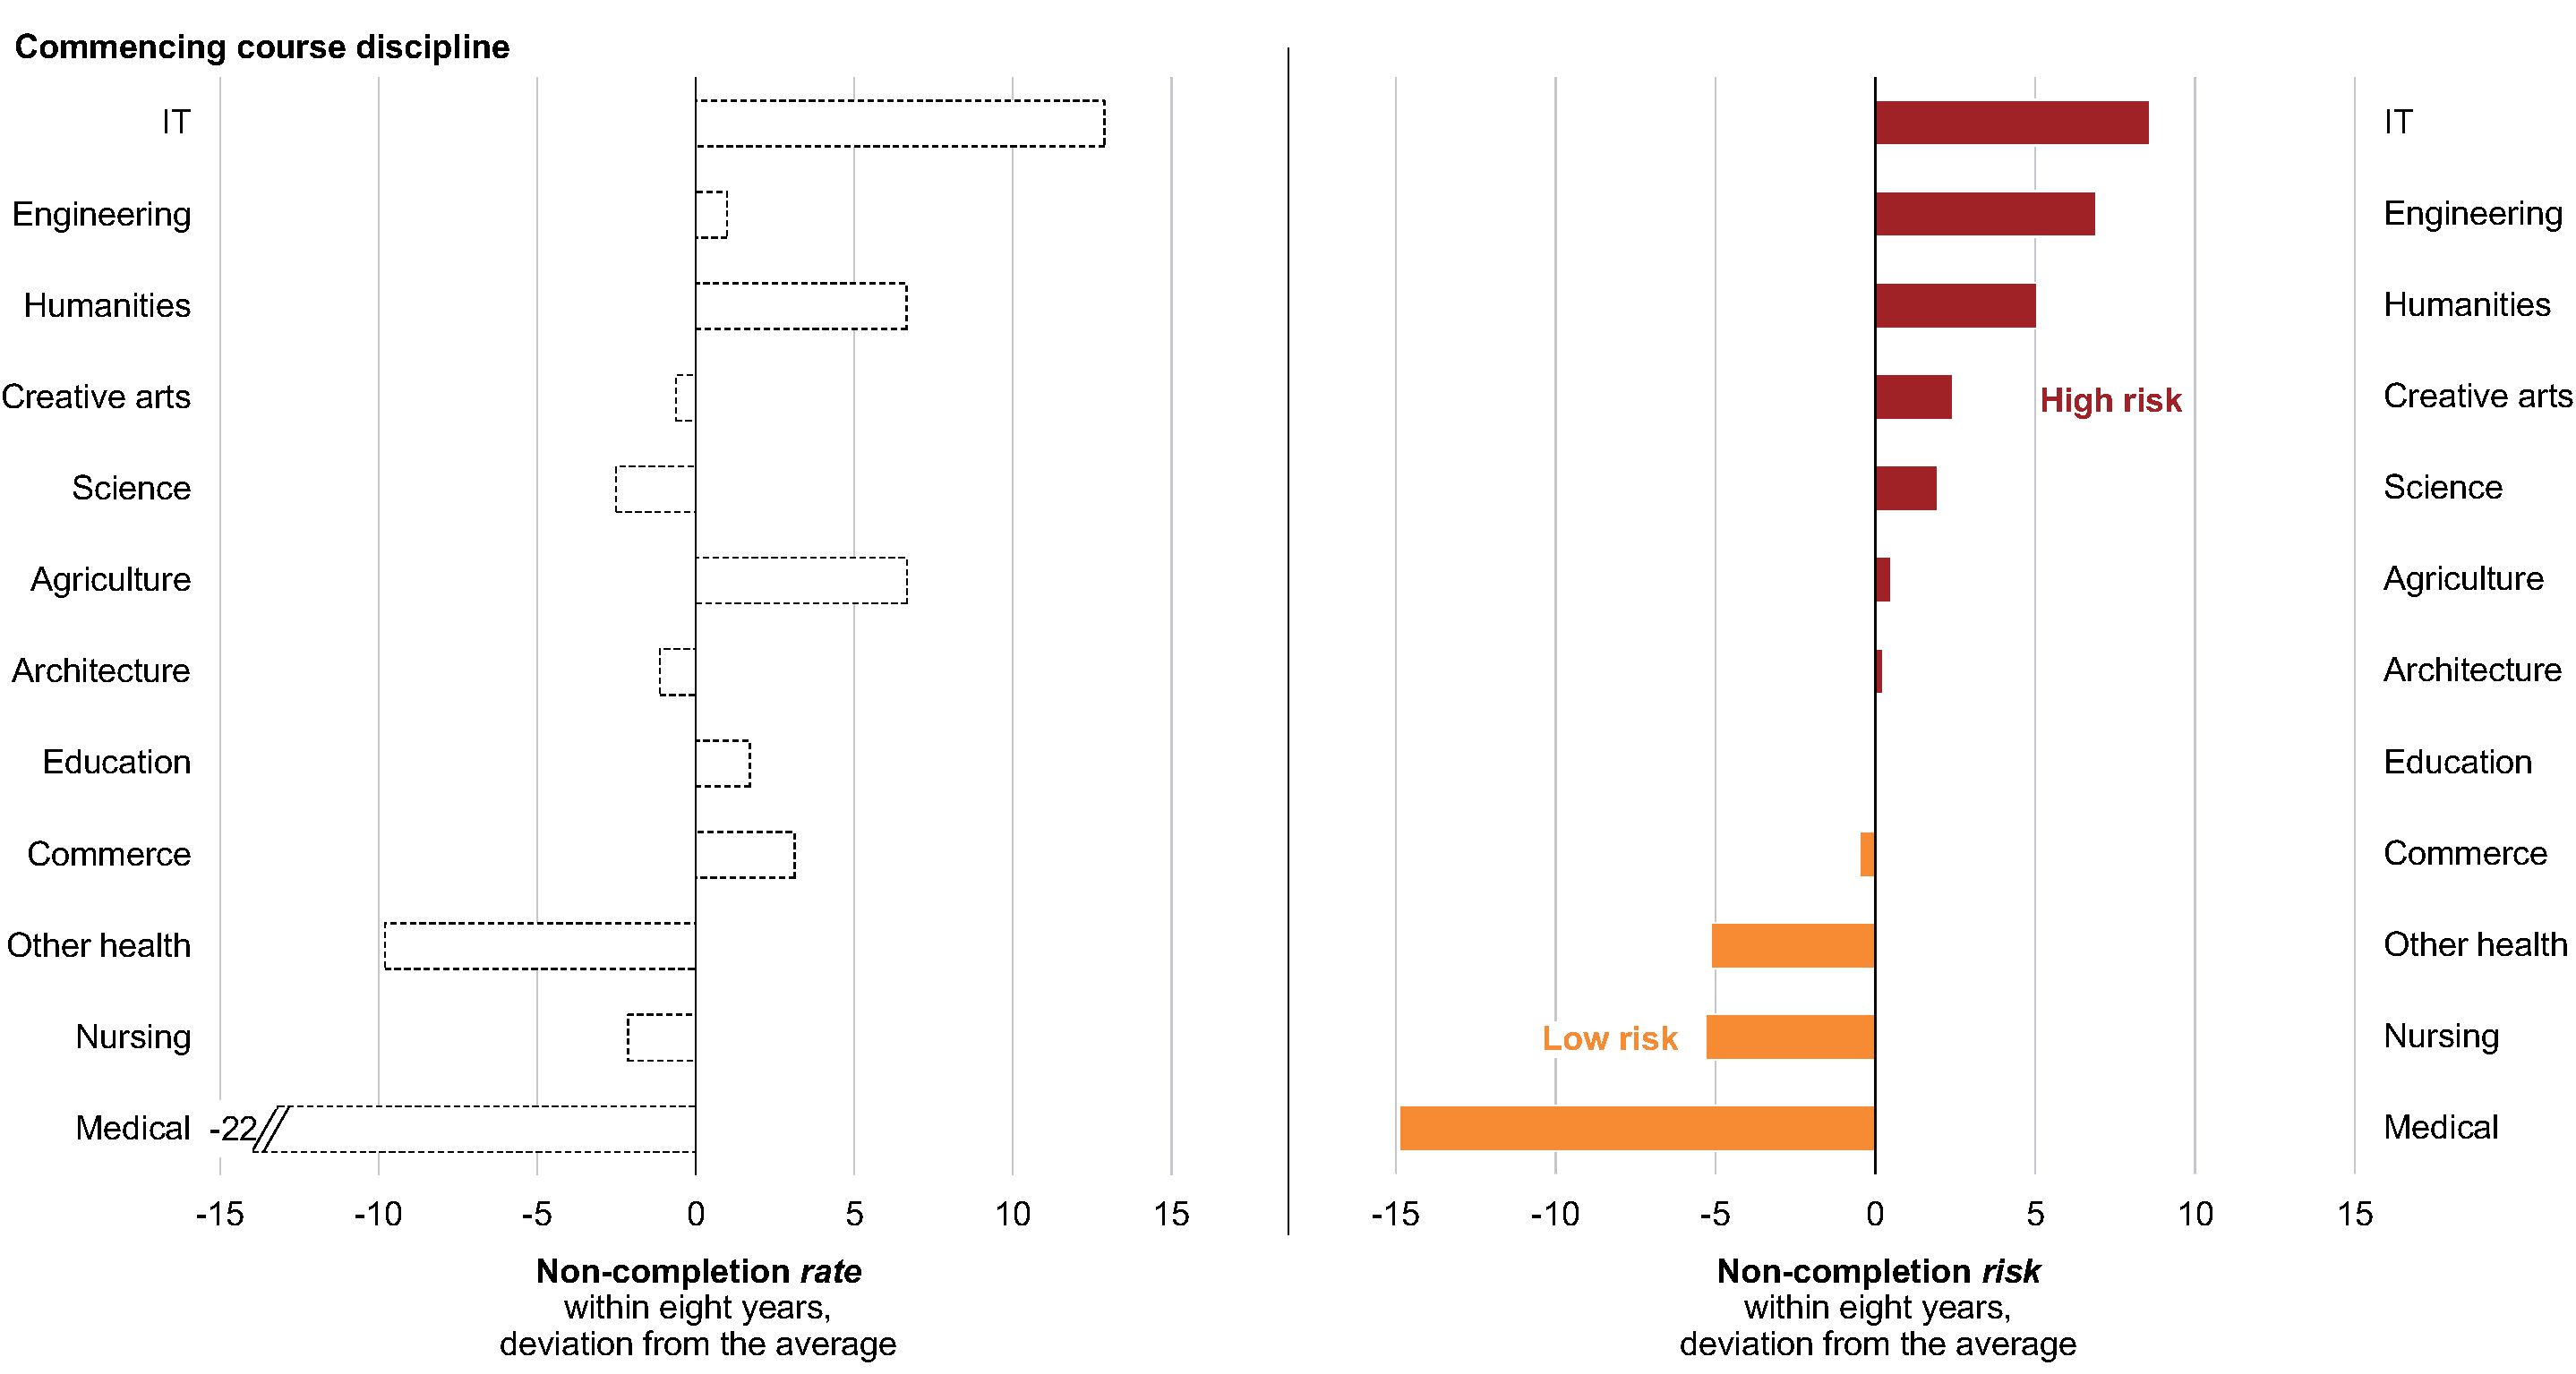
\includegraphics[page=1, width=2.15\columnwidth]{atlas/discipline_fullpage.pdf}
                    \noteswithsource{Discipline of commencing enrolment course. The risk shows deviation from the average rate across fields and universities based on an average person. Law is excluded because it has a much higher share of double-degree students than other disciplines. See also the background paper, \textcite{Cherastidtham2018a}.}
                    {Grattan analysis of \textcite{DepartmentofEducationandTraininga}}
                \end{figure*}

Overall, off-campus students have low rates of completion.\footcite[][table~1]{DepartmentofEducationandTraining2017} 
But after controlling for age, part-time study and other attributes, off-campus study adds only a small amount of risk. On-campus students have a drop-out risk of 31 per cent; for off-campus students it is 33 per cent.

Completion rates vary by the discipline studied, as can be seen in the left side of \Vref{fig:18}. Students in health courses typically have better-than-average completion rates, while IT, humanities and agricultural students do worse than average. These results are influenced by student characteristics -- for example, some courses attract high-ATAR students, with others mostly enrol lower-ATAR students. The right side of \Cref{fig:18} shows the risk of not completing by discipline, after controlling for the ATAR and the other factors in \Vref{fig:table1}. The patterns remain similar, but all the STEM fields (Science, Technology, Engineering and Mathematics) end up with above-average risk, along with humanities and the creative arts. The lowest-risk fields are all health-related. The background paper suggests some possible explanations for this.\footcite[][chapter~4]{Cherastidtham2018a}


\subsection{Equity groups}\label{subsec:3.1.4}

Universities and government have a particular interest in `equity groups', categories of people with a history of lower-than-average higher education attainment. Generally, analysis based on the factors in \Cref{fig:table1} shows that equity group membership is, of itself, associated with only a slightly higher risk of not completing.

On the standard low socio-economic status measure, which is based on the education and occupation levels of people living near the student's home address, completion rates differ little after taking into account other factors.\footnote{Year 12 address for school leavers, permanent home address for others. See \textcite[][section~5.5]{Cherastidtham2018a}.} Students from the top 10 per cent of socio-economic status areas have a 30 per cent risk of not completing; students from the bottom 10 per cent have a 33 per cent risk of not completing.

For students from regional and remote areas, the findings are similar. Compared to students from major cities, students from inner or outer regional areas have the same completion risks, after controlling for other characteristics. Students from remote or very remote areas face an increased risk, of 3 and 6 percentage points respectively. Only small numbers of students come from remote areas.\footnote{For more detail, see \textcite[][section~5.6]{Cherastidtham2018a}.}

Students who report a disability have a non-completion risk 5 percentage points higher than other students. Most students reporting a disability classify it as `medical', although it can be physical, learning or `other'.\footnote{For more detail, see \textcite[][section~5.2]{Cherastidtham2018a}.}

The one equity group with a substantially elevated non-completion risk is Indigenous students. Their risk of not completing is 45 per cent, 15 percentage points above non-Indigenous students. A relatively large proportion of Indigenous students are admitted on an `other' basis, which means that their school results or previous tertiary education were not the main basis for their admission. It's likely that these Indigenous students begin their higher education studies with relatively weak academic preparation.\footnote{For more detail, see \textcite[][section~5.3]{Cherastidtham2018a}.}

Risk results for equity students require careful interpretation. While equity group membership does not of itself usually substantially add to risk, these students are more likely to have other significant risk factors, such as weaker academic preparation or part-time study.\footnote{For the links between ATAR and socio-economic status, see the references at \textcite[][186--188]{Norton2016a}.} 
Socio-economic factors may explain why the student had a relatively low ATAR, or why they need to work full-time and study part-time.

\subsection{Other personal characteristics }\label{subsec:3.1.5}

Where a student was born generally has a modest, 5 percentage points or less, effect on completion prospects. The risk of people born in New Zealand or Asia not completing is slightly higher than for people born in Australia. Similarly, language spoken at home generally has little effect on completion rates. The exception is students speaking an East Asian language such as Chinese at home; their completion prospects are better than those of students who speak English at home.\footnote{For more detail, see \textcite[][section~5.7]{Cherastidtham2018a}.}

Women are more likely to a complete their course than men. After controlling for other factors, men have a 5 percentage points higher risk of not completing than women.\footnote{For more detail see \textcite[][section~5.1]{Cherastidtham2018a}.}

Students who begin their course at age 18 or younger have the lowest non-completion risk, at 28 per cent (\Vref{fig:19}). Risk increases slowly in the early post-school years, and peaks for people beginning their studies between the ages of 21 and 30. The statistical model takes account of the fact that older students are more likely to study part-time, which is the largest non-completion risk. However, even among part-time students, the 20-somethings are less likely to complete than younger or older students.\footnote{For more detail see \textcite[][section~5.4]{Cherastidtham2018a}.}


                % Figure 19
                \begin{figure}
                    \caption{The risk of not completing increases from age 19 to age 30\label{fig:19}}%
                    \units{Risk of not completing within eight years controlling for other factors, per cent}
                    \includegraphics[page=24]{atlas/selection_chartdeck.pdf} 
                    \noteswithsource{Predictive margins are shown. See also the background paper, \textcite[][]{Cherastidtham2018a}.}
                    {Grattan analysis of \textcite{DepartmentofEducationandTraininga}}
                \end{figure}

